\documentclass[border=6pt]{standalone}
\usepackage{tikz}
\usetikzlibrary{arrows.meta,positioning,calc,shapes.geometric,fit,backgrounds,patterns,matrix,decorations.pathreplacing}
\begin{document}
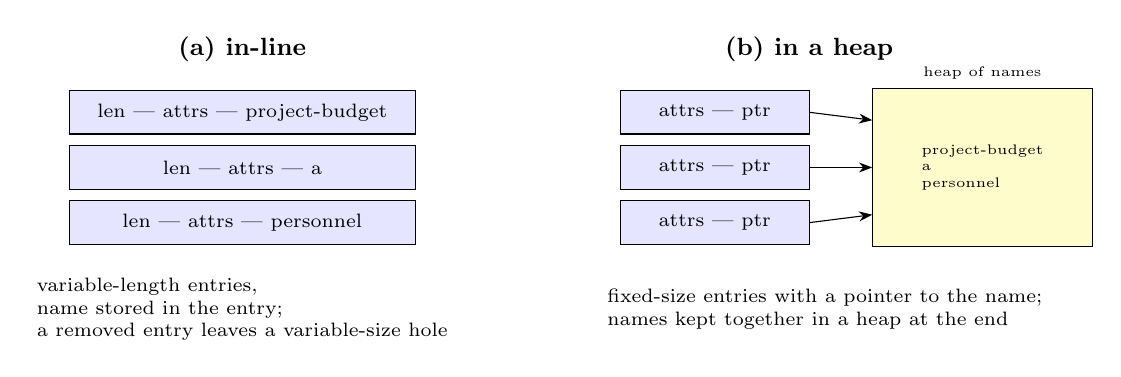
\begin{tikzpicture}[>=Stealth,font=\small]
\tikzstyle{c}=[draw,minimum height=0.55cm,font=\scriptsize]
\node[font=\small\bfseries] at (2.2,2) {(a) in-line};
\foreach \i/\t in {0/{len | attrs | project-budget},1/{len | attrs | a},2/{len | attrs | personnel}} \node[c,minimum width=4.4cm,fill=blue!10] at (2.2,1.2-\i*0.7) {\t};
\node[font=\scriptsize,align=left] at (2.2,-1.3) {variable-length entries,\\ name stored in the entry;\\ a removed entry leaves a variable-size hole};
\node[font=\small\bfseries] at (9.4,2) {(b) in a heap};
\foreach \i/\t in {0/{attrs | ptr},1/{attrs | ptr},2/{attrs | ptr}} \node[c,minimum width=2.4cm,fill=blue!10] (e\i) at (8.2,1.2-\i*0.7) {\t};
\node[c,minimum width=2.8cm,minimum height=2.0cm,fill=yellow!20] (h) at (11.6,0.5) {};
\node[font=\tiny,align=left] at (11.6,0.5) {project-budget\\ a\\ personnel};
\node[font=\tiny] at (11.6,1.7) {heap of names};
\draw[->] (e0.east) -- (10.2,1.1); \draw[->] (e1.east) -- (10.2,0.5); \draw[->] (e2.east) -- (10.2,-0.1);
\node[font=\scriptsize,align=left] at (9.6,-1.3) {fixed-size entries with a pointer to the name;\\ names kept together in a heap at the end};
\end{tikzpicture}
\end{document}
